In this chapter a general overview of our software to be and its functionalities is given. In section \ref{sec:product_perspective} we will present a conceptual model of the domain we are working in, where, in addition to the real world objects that are significant in our domain and to our system, we include the main components of our system that will interface with the environment. Then, we proceed by presenting the state diagrams of the most important scenarios discussed in the following subsection. In section \ref{sec:Product functions} we give a description of the main functionalities our system has to provide, but without going in much detail since we will delve into this aspects in the next chapter. In section \ref{sec:User_characteristics} we provide an analysis of the target users of the system, which are the clients that will use the system or will interact with it. Finally, in section \ref{sec:Assumptions, dependencies and constraints}, we outline the assumptions, the dependencies and the constraints, necessary to be taken into account when implementing the software.
\section{Product perspective}
\label{sec:product_perspective}%
\subsection{Domain model}
We start off this chapter by analyzing the domain model (or \textit{conceptual model}) we came up with to represent the domain we are working in. Being a conceptual model the diagram was not drafted with all the formalism specified in the UML notation; we actually used a pretty informal description, specifying multiplicity and reading direction only when strictly necessary. The model in figure \ref{domain_model} was drawn using the UML class diagram notation, and illustrates only the conceptual classes that are significant to the domain \cite{larmanUML}. We also included the classes representing the component of our system to be that will interact directly with the environment.\\
\begin{figure}[H]
    \centering
    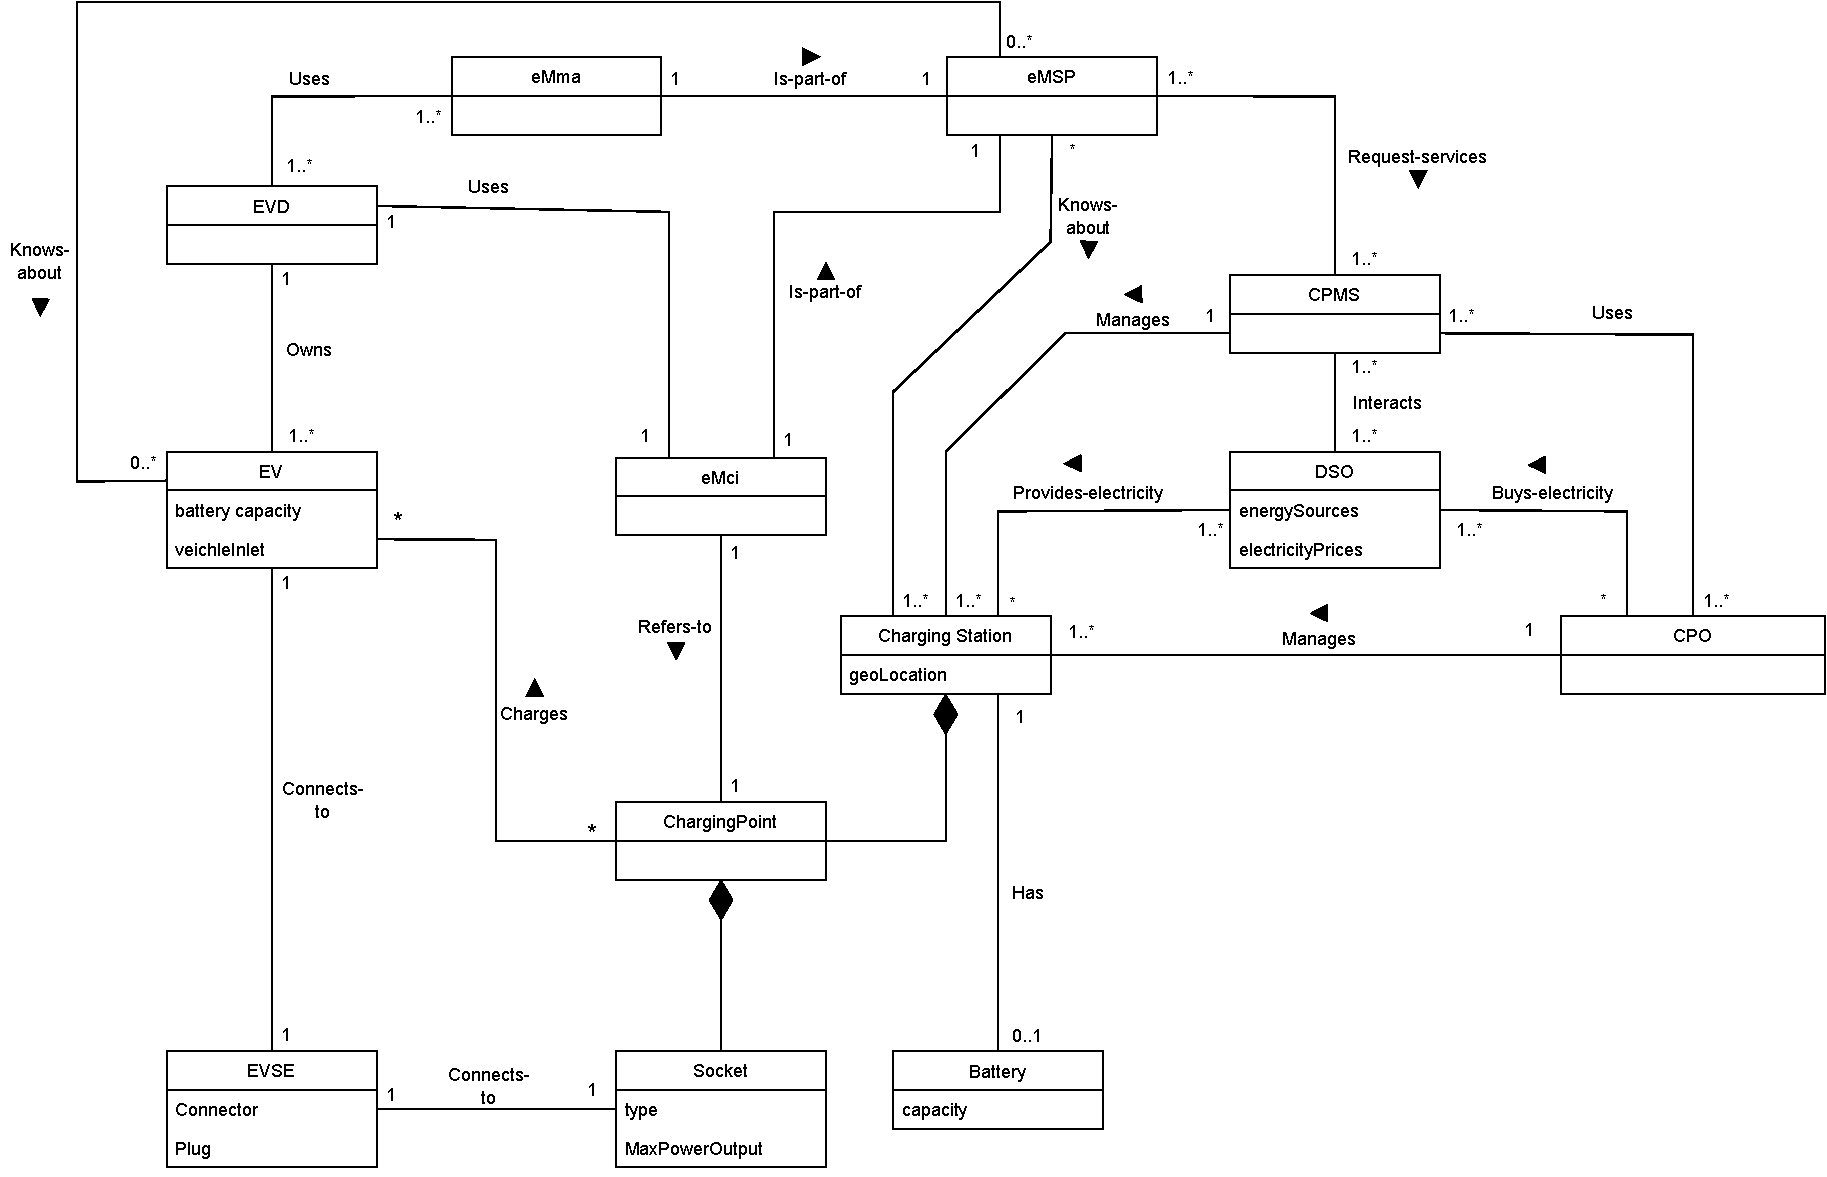
\includegraphics[width=1\textwidth]{Images/cp2/domain_model_v1}
    \caption{Domain model}
    \label{domain_model}
\end{figure}

We now proceed discussing some of the elements that may not be so immediate only by reading the domain model.


\paragraph{EVSE}
The EVSE, as mentioned in \ref{sec:Definitions, Acronyms, Abbreviations}, is a general term that refers to the the equipment that allows a vehicle to be recharged. In this context we can see it as a universal adapter that can be an interface for the vehicle inlet and the socket of the charging point. In the diagram this is shown by the association \textit{'Connects-to'} for both class EV and Socket. The multiplicity one-to-one for both associations is to show that at a specific moment a vehicle can be connected to a socket only through one single EVSE \cite{larmanUML}. Obviously, an EV can connect to all the EVSEs that have a connector compatible with its inlet, and a Socket can connect to all the EVSEs that have a compatible plug. It also should be noticed that there are charging points that do not expose the socket directly, but they have an integrated EVSE, namely a cable with it's connector.

\paragraph{DSO}
In the model the DSO is represented as interacting with both CPO and the CPMS. This happens because we do not distinguish between the actual business and the Information System he uses. So the association between DSO and CPMS is to be intended as the interaction between the two software systems, meanwhile, the association between DSO and CPO represents the interaction of the two businesses.

\paragraph{ChargingPoint}
This class represents the actual physical device that contains the sockets to which the EV will connect to charge.

\paragraph{Battery} In the association \textit{'Has'} between ChargingStation and Battery we have stated that an instance of ChargingStation may have only one Battery. The reason behind this decision is that we opted for a high level of abstraction and with the class Battery we intend a generic energy storage, without concerning ourselves with the actual physical properties or requirements of the item itself.

\paragraph{CPO} The multiplicity one-to-many in the association \textit{'Uses'} between CPO and CPMS is motivated by our view of the system. In our perspective, the CPMS is viewed as a software that is offered to different businesses that manage their charging stations, thus a business through the CPO can choose to manage the charging stations with different CPMS systems.

\subsection{State charts}
Among the main interactions with the eMall we have decided to represent here with state diagrams the ones that we consider the most interesting and complex uses of the system, from EVD point of view: the initiation of a charging session and the booking operation.

\begin{figure}[H]
    \centering
    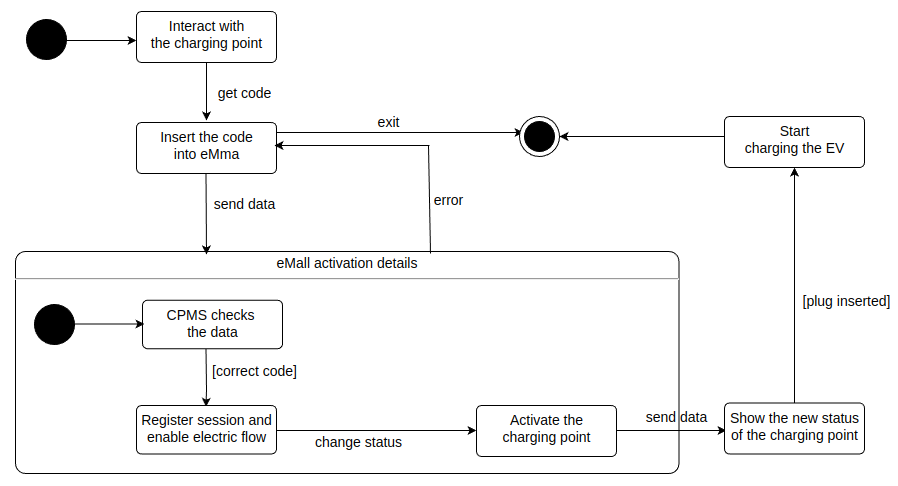
\includegraphics[width=0.95\textwidth]{Images/ChargingNow.png}
    \caption{State diagram of the EVD that starts a charging session}
\end{figure}

\begin{figure}[H]
    \centering
    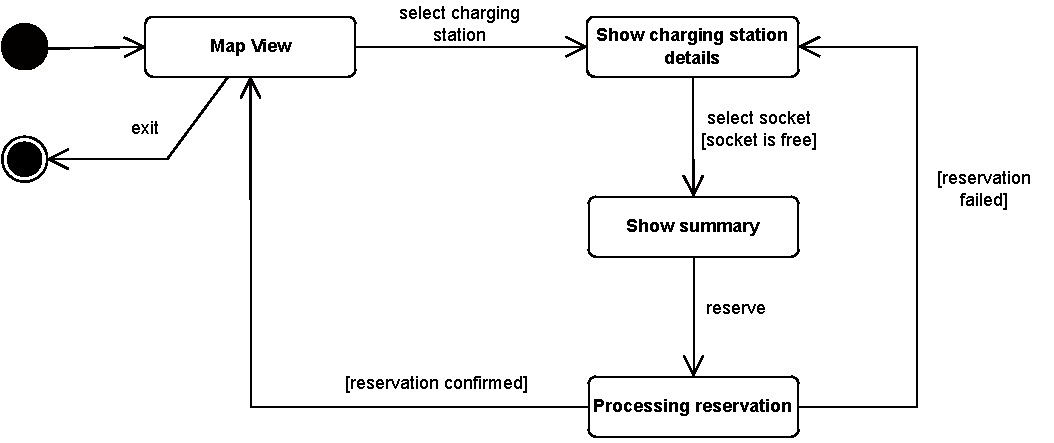
\includegraphics[width=0.85\textwidth]{Images/booking_charge_state_diag}
    \caption{State diagram of the EVD that books a charging point}
\end{figure}

We also report another state diagram to represent the main interaction of the CPO with the managerial part of our software. We consider the case in which the CPO wants to modify some parameters regarding a certain charging station. 

\begin{figure}[H]
    \centering
    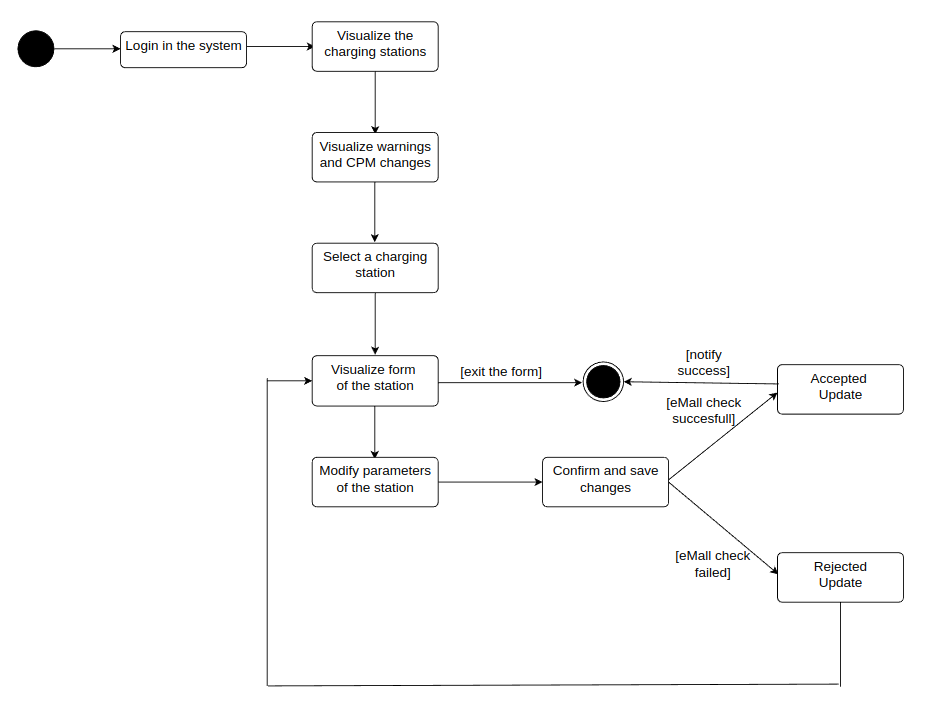
\includegraphics[width=0.95\textwidth]{Images/CPOparams.png}
    \caption{State diagram of the CPO that manages charging stations}
\end{figure}

\subsection{Scenarios}
\paragraph{Booking a charging point}
Edward, after getting in his electric vehicle, notices that the battery is at low percentage, so he plans to book a charge at a station nearby. He grabs his smartphone and opens the mobile app eMma to look for a charging station. When Edward opens the app he is greeted with the view of a map showing him the nearest charging stations to his location. The charging stations are represented with icons of different colors. The colors are used to distinguish totally occupied charging stations from those with free sockets that can be used to charge an EV. After moving around the map, Edward finds a charging station with free sockets suitable to his needs. He clicks on the icon symbolizing the charging station and a new view is drawn on the screen. The view visualizes information about the specific station, namely:
\begin{itemize}
    \item the name of the charging station
    \item the rating of the charging station
    \item indication about the available sockets types
    \item contact details
    \item address of the charging station
    \item any directions on how to handle the charging process
    \item reviews relative to the charging station
\end{itemize}
Edward, being satisfied with the characteristics presented by the station, clicks on the button 'Book now' opening yet another view, which lists all the available sockets, pointing out the following information for each one of them:
\begin{itemize}
    \item the type of charging (AC/DC)
    \item the type of the socket (type 1, type 2, CCS, CHAdeMO, etc.)
    \item the charging speed denoted in kW and km/h (km gained per one hour of charge)
    \item the price for kWh
    \item the price for unlocking the socket
\end{itemize}
Scrolling down on the app, additional information regarding the station and the charging process are shown, like:
\begin{itemize}
    \item accessibility to the station
    \item any additional fees set by the CPO, such as the cost per minute for parking during the charging process and the cost per minute for parking after finishing the charging (penalty for occupying the spot and not using it)
    \item taxation information (VAT etc)
\end{itemize}
Being satisfied by the features offered by this station, Edward selects the appropriate socket for his EV and equipment (any additional charging adapter) and inserts the time-frame (date and time) in which he wants to reserve the spot.


\paragraph{Update profile details}
Jay is an electric vehicle enthusiast, who bought himself a new EV in order to reduce the negative impact on the environment. Given this new purchase, Jay needs to update his profile on the eMma in order to take advantage of the eMall service at its most. He logs in to his account on the mobile app and from the main page navigates to his profile. On the profile page are visible the personal information and the details about the EVs. On the page there is also the button that allows to update the profile and this is exactly what Jay is looking for. After pressing the button 'Update' there are different possibilities and Jay chooses the one that states 'Add new vehicle'. Now he has to fill up a form with the EV's details, such as type, capacity of the battery, supported power and electircal current and so on. After double checking the form, Jay presses the 'Ok' button and the page reloads showing again the profile page that now states among the other vehicles also the new one. Considering the eventuality of making mistakes in completing the form it is always possible to come back to the EV details and change any present field.

\paragraph{Visualize charging history}
It has been nearly 6 months since Hannah bought her first EV and now she has fully grasped how the whole ecosystem around it works. In the past few months Hannah has tried quite a few different charging stations to explore how each one is managed and organized. Having tried all these charging stations Hannah is curious to see how many charging stations she has visited, how frequently and how much she has paid for the charging. With this objective in mind Hannah opens the eMma application in her mobile phone and heads to the history section of it. This section is divided in two parts: in the top half the app shows the imminent charging booking that Hannah has reserved, if present. In the bottom half of the screen, the app shows a chronologically ordered list of all the charges processed through eMma. Each entry in the list shows the date in which the charging was done, where it was done, for how long, how many kWh were charged, the type of the socket used and how much did it cost distinguishing between cost for kWh and total cost. Hannah can also choose a different visualization for the charging history, filtering it based on some criteria (EV, time-period, location).

\paragraph{Start a charging session}
Adeline usually goes to the supermarket nearer to her house because it has a charging station in the parking area. Most of the times she finds an available charging point so she charges her EV while she does the grocery. Once stopped the car in the available spot Adeline wants to start a charging session. She interacts with the charging point interface, visualizes the information about the available charge with the respective power and cost and inserts the code shown on the screen in the mobile app of the eMall, the eMma. Once initiated the session from the mobile phone, the data are sent to the system, and in particular to the CPMS part of the software that checks the correctness of the inserted code and registers the session related to the user. Then, the CPMS enables the flow of electricity in order to actualize the charging from the charging point. If during the check of the data and during the activation operations there are no errors the status of the charging point changes and the session is activated. Now, Adeline can insert the specific plug, compatible with her car, in the EV in order to actually start the charging, which if not stopped earlier will terminate when the battery is full.

\paragraph{A new user registers into eMma}
Michael, proud owner of an EV for 5 years, has decided to try this new charging app, eMma, that is promoting itself as a better alternative to manage in a smart way the charging process of an EV. Michael decides to give eMma a chance, downloads the app and immediately initiates the procedure to create a new account. The first phase of the registering process is straightforward; the usual information about name, surname, email and password are requested. After completing this first phase eMma prompts the user with a message asking him the consent to use his geographical location and to accept the terms of service. Micheal gladly accepts because he wants the app to show him the charging station nearest to him based on his location. After granting the consent a new page is presented to Michael. This time it is a form to be completed with the information about Michael’s EVs specifications and his EV equipment, like charging adapters and cables. Michael understands that this information is needed so the app can work in a smart way, showing him only the charging stations that have sockets compatible with Michael EVs connector or adapters. Finally the process to complete the registering begins; a form where Michael has to add his electronic payment details. After completing this last stage, the app opens and shows Michael a map of the area around him where the charging stations are highlighted with icons of bright colors.


\paragraph{Visualize the charging stations map}
Daisy is an unusual user of the eMall, that didn't registered an account. Anyway the system allows the possibility to use the application as a guest, but the functionalities are limited. Daisy is only interested in visualizing the charging stations nearby, so she opens the main page of the app in order to look at the map. The system retrieves, based on the location shared by the phone, the charging stations in the area and shows them on the map. Daisy can now explore the charging stations around clicking on them on the map, and she can see their rating with the relative reviews and can choose the service that better fits her needs. She can visualize the price and the available chargers with their type of connectors, but she is not able to book a charging session without an account. Once identified her preferred charging station Daisy closes the application, gets in her car and heads directly to charge her EV.

\paragraph{Manage the charging stations}
Nick is a CPO that on a typical day has to monitor the charging stations assigned to his department. After arriving to work and logging in the system with the company credentials Nick checks the list of charging stations and any new notification given by the CPMS part of the eMall about the DSOs decisions. He sees a warning regarding the recently deployed charging station in Rome and clicking on it the web application of the eMall shows a form with the various characteristics of the station. The parts that may have undergone a modification are highlighted in red and in this case the selection of the DSO has new options available and Nick clicks on it to explore the more convenient ones. He notices a change in one of the DSOs that now grants energy also through renewable resources, and given the green policy of the company he chooses this new kind of supply. Considering the price of 0.036/kWh provided by the DSO, in order to have a profit, according to the business modus operandi Nick sets the cost charging at 0.040/kWh. Once confirmed the DSO from which to acquire energy by looking carefully at the form he becomes aware of the fact that at the moment there are no EVD charging at the station and also sees that there are available batteries in which to store energy. One of the batteries is empty, so he selects it in order to store energy in it right away, until the full capacity C, given the off-peak moment. After all this operations Nick saves the changes and the eMall notifies him about the success of the procedure, that has an immediate effect on the system and his interaction with the world. Nick moves on to the next charging station of his list, checking up in similar way each one of the stations for which he is responsible. 



\section{Product functions}
\label{sec:Product functions}%
In this section, we briefly represent a list of the most important requirements of the \verb|eMAll|, remainig on a high level of abstraction, since we will proceed to further discuss about them in much more detail in the next chapter.
\subsection{Data collection and management}
One of the main functionalities of the software is to store and manage different kinds of data coming from different sources:
\begin{enumerate}
    \item The EVD using the eMma inserts into the system different kind of data. He inserts personal data, such as name, surname, and payment details; he also adds information about his EVs, like the maximum and minimum current supported, the connector type, the battery capacity and other relevant facts, like any additional EVSE he might own. The eMall allows the insertion of structured data and full-text elements that are subjected to checks in order to verify their correctness. The software maintains these data on the database in order to associate the bookings and the charging sessions to all registered EVDs, who can access all the functionalities of the system and are not subjected to the payment of a deposit every time they use a charging point
    \item The DSO provides energy to the charging stations, and the information about the DSO's supply is automatically collected by the CPMS subsystem of the eMall through interfaces that interact with the external systems. The CPMS acquires the information and saves it on the database in order for it to be visible to the CPO, and updates these data periodically. The collected data deriving from the DSO's are essential for the businesses, which make their supply choices depending on the price, the availability and the kind of acquired energy 
    \item The CPO manages the charging stations and their supply, visualizing the information kept by the software and making data-driven decisions for each one of the charging stations owned by the company. The CPO can see the parameters of each station and change them based on the new prices and types of energy, based on the chosen DSO to acquire from and based on the new politics of the CPO's company. All the data updates done by the CPO are received by the CPMS and collected by the system, so the managerial part of the service constantly produces data, about the charging stations. These data are stored and then used by the software to inform the EVDs of the charging stations details. The eMall also keeps data about the charging points and about the presence of batteries in each charging station, and these are useful information that need to be collected in order to allow to the CPOs to manage the service accurately
    \item The charging station itself is an important source of data. Information about the charging points usage, both in terms of frequency throughout different periods of time (day, week, month) and usage time (for how long a certain socket has been used for each charging process) must be kept to enable the eMall system to conduct data analysis procedures (can give information about peak load hours) and empower the CPOs with relevant data for the business decision making process. Other information that can be tracked through the system include: client profiling (keep track of clients who visit the charging station), maintenance record, unused bookings profile
\end{enumerate}

\subsection{Communication and knowledge sharing}
The eMall provides different tools to the EVD and to the CPO in order to take advantage of the service and obtain all the needed information from the system.. To be able to share this knowledge the subsystems of the software need to communicate among themselves and with the external entities. The offered tools are the following:
\begin{enumerate}
    \item The eMma presents to the EVD all the information needed about the nearby charging stations. The application shows a map with the charging stations, and selecting a station the user can visualize further data, such as price, socket type, free charging points and other details. The eMma and the eMci are able to provide these information, because are part of the eMSP, which communicates with the CPMS to acquire the data about the charging stations 
    \item The web app available to the CPO, communicates with the CPMS part of the software getting the data about the electric supply offered by the DSOs, acquiring knowledge about the prices, the special offers and the available electric sources. The CPMS updates the information interacting periodically with the external service of the DSOs and shares the knowledge with the CPO
\end{enumerate}
It is evident that among the functionalities of knowledge sharing and communication between the components involved, we also have as main features the following:
\begin{enumerate}
    \item The eMma shows to the EVD the information about the nearby charging stations
    \item The eMci shows to the EVD the data regarding the charging point in use
    \item The CPMS gives to the CPO the knowledge of the DSOs changes and the last data saved for each charging station managed by the CPO
\end{enumerate}

\subsection{Main functionalities}
Regarding the main functionalities that the EVD perceives, except for the ones already described, the most important ones remain:
\begin{enumerate}
    \item The eMma allows to the EVD to book a charging point in a chosen time frame. Once the booking is completed from the app, the EVD receives a confirmation notification and the booking with an associated code is added to the user history of charges. The system saves the data related to the registered EVD and to the booking, so the eMSP maintains a copy of the code provided to the user, the data associated to the charging station and the chosen time frame. The effective charging service will be provided when the user will correctly insert the received code into the che eMci of the specific charging point. The eMall, after checking the code, activates a charging session with respect to the EVD, having in this way that the system provides the functionality of charging the EV in the time frame previously booked
    \item The eMall gives, also, the possibility to charge without booking. In this case the EVD interacts  with the eMma and the eMci. From the two interfaces the data arrive to the eMSP, which creates the charging session and allows the user to use the service
\end{enumerate}

\section{User characteristics}
\label{sec:User_characteristics}%
The eMall has three main user classes:
\begin{enumerate}
    \item \textbf{Unregistered EVD}: An EVD can register to the eMall or use the service without registration. In order to register, the user has to introduce personal data and the details of the EVs, so he creates a profile with an associated name and a password. By creating a profile is possible to take advantage of all the features provided by the service, having some privileges, but the eMall can also be used without any registration. The eMma can be downloaded on the phone and used as a 'guest' and in this case is still possible to visualize the map with all the nearby stations and their information. It is also possible to book a charging session from the application, but is necessary at least the insertion of the payment details and the payment of a deposit in advance in order to use this functionality. Even in the case of charging the EV without any booking, the unregistered EVD has to give a deposit before starting the charging session. Furthermore, the EVD without a profile doesn't have the history of charges, so there are some limitations in using the system
    \item \textbf{Registered EVD}: An EVD is registered if creates an account inserting personal data and EVs details. The registered EVD interacts with the eMma and the eMci in order to use the main functionalities of the system: to book a charging session, to charge the EV without a booking, to visualize the nearby charging stations and to visualize and modify the personal profile and history. The EVD, registered or unregistered, can be unfamiliar with the use of mobile applications, so the software needs to be user-friendly in order to guarantee a good service in all its aspects 
    \item \textbf{CPO}: A company that supplies the service is identified with the employees or the existing software, that interacts with the eMall system. In the interaction the part of the company is called the CPO and manages the charging stations provided by the company itself. The CPO is able to visualize all the stations and the respective charging points and can change the supply parameters, modifying the price of the charge, the storage of energy, the DSOs from which to acquire electricity and other details. All these changes are possible given the interaction of the CPO with the CPMS part of the eMall, which has the necessary knowledge, that is communicated to the company in order to administer the stations and offer the service properly 
\end{enumerate}

\section{Assumptions, dependencies and constraints}
\label{sec:Assumptions, dependencies and constraints}%
Here we report the main domain assumptions used for the modeling of the eMall. We tried to leave as much freedom as possible, not liming the system with too much assumptions.
\newcounter{ac}
\setcounter{ac}{1}
\newcommand{\acount}{\theac\stepcounter{ac}}
\begin{table}[h!]
    \centering
    \begin{tabular}{|l|p{0.725\linewidth}|}
     \hline
     \textbf{Assumptions} & \textbf{Description} \\
     \hline
     D\acount & The EVD has internet connection \\
     \hline
     D\acount & The EVD has a mobile phone with an integrated GPS module \\
     \hline
     D\acount & The EVD has the mobile application of the eMSP installed on his mobile phone \\
     \hline
     D\acount & The EVD inserts correct data in the mobile application \\
     \hline
     D\acount & The CPO inserts correct data in the web application \\
     \hline
     D\acount & The CPOs send the data of the charging stations to the eMall \\
     \hline
     D\acount & The end user payment from the mobile app is handled by external APIs.\\
     \hline
     D\acount & The EVD that creates an account inserts the personal data and the payment details during registration \\
     \hline
     D\acount & The CPO uses company credentials to access the web application of the eMall \\
     \hline
     D\acount & The DSO is associated to the whole charging station \\
     \hline
     D\acount & There is a type of promotion, that can be associated to the whole charging station \\
     \hline
     D\acount & There is a type of promotion, that can be associated to only a charging point \\
     \hline
     D\acount & The price can vary in different charging points \\
     \hline
\end{tabular}
    \caption{Assumptions}
    \label{tab:Assumptions}
\end{table}